\chapter{Ejercicios de clase}
\noindent
Esta sección tiene el propósito de recoger todos los ejercicios propuestos en clase por parte de la profesora y que fueron resueltos por los alumnos en pizarra.

\section{Estadísticos muestrales}
\begin{ejercicio}
    Obtener la función masa de probabilidad conjunta de una m.a.s. de $X\rightsquigarrow B(k_0,p)$ y la función de densidad de una m.a.s. de $X\rightsquigarrow U(a,b)$.\\

    \noindent
    Recordamos que si $X\rightsquigarrow B(k_0, p)$, entonces:
    \begin{equation*}
        P[X = x] = \binom{k_0}{x} p^x{(1-p)}^{n-x} \qquad \forall x\in \{0,\ldots,k_0\}
    \end{equation*}
    Por lo que si tenemos una m.a.s. de $n$ variables independientes e idénticamente distribuidas a $X$, $(X_1, \ldots, X_n)$, su función de densidad vendrá dada por:
    \begin{align*}
        P[X_1 &= x_1, \ldots, X_n = x_n] \stackrel{\text{indep.}}{=} \prod_{i=1}^{n}P[X_i = x_i]\stackrel{\text{id. d.}}{=} \prod_{i=1}^{n} P[X=x_i] \\
              &= \prod_{i=1}^{n} \binom{k_0}{x_i} p^{x_i} {(1-p)}^{k_0-x_i} = p^{\sum\limits_{i=1}^{n}x_i} {(1-p)}^{nk_0 - \sum\limits_{i=1}^{n}x_i} \prod_{i=1}^{n}\binom{k_0}{x_i} \\
              & \qquad \forall x_i \in \{0,\ldots,k_0\}
    \end{align*}

    \noindent
    Si ahora $X\rightsquigarrow U(a,b)$ para ciertos $a,b\in \mathbb{R}$ con $a<b$, entonces:
    \begin{equation*}
        f_X(x) = \dfrac{1}{b-a} \qquad \forall x\in [a,b]
    \end{equation*}

    de donde:
    \begin{equation*}
        f_{(X_1, \ldots, X_n)}(x_1, \ldots, x_n) \stackrel{\text{indep.}}{=} \prod_{i=1}^{n} f_{X_i}(x_i)\stackrel{\text{id. d.}}{=} \prod_{i=1}^{n} f_X(x_i) = \prod_{i=1}^{n} \dfrac{1}{b-a} = \dfrac{1}{{(b-a)}^{n}} \qquad \forall x\in [a,b]
    \end{equation*}
\end{ejercicio}

\begin{ejercicio}
    Para cada realización muestral, $(x_1, \ldots, x_n)\in \cc{X}^n$, $F_{x_1,\ldots,x_n}^\ast$ es una función de distribución en $\mathbb{R}$. En particular es una función a saltos, con saltos de amplitud $\nicefrac{1}{n}$ en los sucesivos valores muestrales ordenados de menor a mayor, supuestos que sean distintos, y de saltos múltiplos en el caso de que varios valores muestrales coincidieran.\\

    \noindent
    En las condiciones del enunciado, es decir, suponiendo que $x_1, \ldots, x_n$ están ordenados de menor a mayor y son distintos, entonces es fácil ver que:
    \begin{equation*}
        F_{x_1, \ldots, x_n}^\ast (x) = \left\{\begin{array}{ll}
                0 & \text{si\ } x < x_1 \\
                \nicefrac{1}{n} & \text{si\ } x_1 \leq x < x_2 \\
                                &\vdots \\
                            1 & \text{si\ } x > x_n
        \end{array}\right. \qquad \forall x\in \mathbb{R}
    \end{equation*}
    Por lo que es claro que $F_{x_1, \ldots, x_n}^\ast $ es no decreciente, continua por la derecha, con límite 0 en $-\infty$ y con límite 1 en $+\infty$.
\end{ejercicio}

\begin{ejercicio}
    $\forall x\in \mathbb{R}$, $F_{X_1, \ldots, X_n}^\ast(x)$ es una variable aleatoria tal que \newline $nF_{X_1, \ldots, X_n}^\ast(x) \rightsquigarrow B(n,F(x))$ y:
    \begin{equation*}
        E[F_{X_1, \ldots, X_n}^\ast (x)] = F(x), \qquad Var[F_{X_1, \ldots, X_n}^\ast (x)] = \dfrac{F(x)(1-F(x))}{n}
    \end{equation*}
    donde $F(x)$ es la función de distribución de $X$.\\

    \noindent
    Recordamos que:
    \begin{equation*}
    F_{X_1, \ldots, X_n}^\ast (x) = \dfrac{1}{n}\sum_{i=1}^{n}I_{\left]-\infty,x\right]}(X_i) \qquad \forall x\in \mathbb{R}
    \end{equation*}
Fijado $x\in \mathbb{R}$, tenemos que $I_{\left]-\infty,x\right]}(X)\rightsquigarrow B(1,P[X\leq x]) \equiv B(1,F(x))$, por lo que por la propiedad reproductiva de la binomial tenemos que:
    \begin{equation*}
        nF_{X_1, \ldots, X_n}^\ast (x) \rightsquigarrow B(n,F(x))
    \end{equation*}
    Por lo que:
    \begin{equation*}
        nE[F_{X_1, \ldots, X_n}^\ast (x)] = E[nF_{X_1, \ldots, X_n}^\ast (x)] = nF(x)
    \end{equation*}

    de donde:
    \begin{equation*}
        E[F_{X_1, \ldots, X_n}^\ast (x)] = F(x)
    \end{equation*}
    Para la varianza:
    \begin{equation*}
        n^2Var[F_{X_1, \ldots, X_n}^\ast (x)] = Var[nF_{X_1, \ldots, X_n}^\ast (x)] = nF(x)(1-F(x))
    \end{equation*}
    
    de donde:
    \begin{equation*}
        Var[F_{X_1, \ldots, X_n}^\ast (x)] = \dfrac{F(x)(1-F(x))}{n}
    \end{equation*}
\end{ejercicio}

\begin{ejercicio}
    Para valores grandes de $n$, en virtual del Teorema Central del Límite:
    \begin{equation*}
        F_{X_1, \ldots, X_n}^\ast (x) \rightsquigarrow \cc{N}\left(F(x), \dfrac{F(x)(1-F(x))}{n}\right)
    \end{equation*}

    \noindent
    Sea $(X_1, \ldots, X_n)$ una m.a.s. de $n$ muestras, sea:
    \begin{equation*}
        S_n = \sum_{i=1}^{n} I_{\left]-\infty,x\right]}(X_i) \qquad \forall n\in \mathbb{N}
    \end{equation*}
    Por el Teorema Central del Límite tenemos que:
    \begin{equation*}
        \dfrac{S_n - E[S_n]}{\sqrt{Var[S_n]}} \stackrel{n\to \infty}{\rightsquigarrow} \cc{N}(0,1) \Longrightarrow S_n \stackrel{n\to \infty}{\rightsquigarrow} \cc{N}\left(F(x), \dfrac{F(x)(1-F(x))}{n}\right)
    \end{equation*}
    Como $S_n \rightsquigarrow B(n,F(x))$, entonces tenemos que:
    \begin{align*}
        E[S_n] &= nF(x) \\
        Var[S_n] &= nF(x)(1-F(x))
    \end{align*}
    Por lo que:
    \begin{equation*}
        F_{X_1, \ldots, X_n}^\ast (x) = \dfrac{1}{n}S_n \stackrel{n\to \infty}{\rightsquigarrow} \cc{N}\left(F(x), \dfrac{F(x)(1-F(x))}{n}\right)
    \end{equation*}
\end{ejercicio}

\begin{ejercicio}
    Dada una muestra aleatoria simple formada por las observaciones $(3, 8, 5, 4, 5)$, obtener su función de distribución muestral y realizar la representación gráfica.\\

    \noindent
    Aplicando la definición de la función de distribución muestral obtenemos que:
    \begin{equation*}
        F_{(3, 8, 5, 4, 5)}^\ast(x) = \left\{\begin{array}{ll}
                0 & \text{si\ } x < 3 \\
                \nicefrac{1}{5} & \text{si\ } 3 \leq x < 4 \\
                \nicefrac{2}{5} & \text{si\ } 4 \leq x < 5 \\
                \nicefrac{4}{5} & \text{si\ } 5 \leq x < 8 \\
                1 & \text{si\ } x \geq 8 
        \end{array}\right.
    \end{equation*}

    \begin{figure}[H]
        \centering
        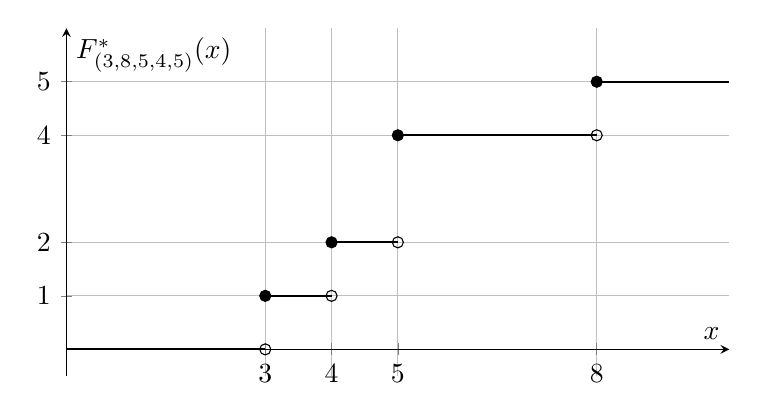
\begin{tikzpicture}
        \begin{axis}[
            axis lines=middle,
            xlabel={$x$},
            ylabel={$F_{(3,8,5,4,5)}^\ast (x)$},
            ymin=-0.5, ymax=6,
            xmin=0, xmax=10,
            xtick={3,4,5,8},
            ytick={0,1,2,4,5},
            grid=both,
            width=10cm,
            height=6cm
        ]

        % Tramos de la función
        \addplot[domain=0:3, thick] {0};

        \addplot[domain=3:4, thick] {1};
        \addplot[domain=4:5, thick] {2};
        \addplot[domain=5:8, thick] {4};
        \addplot[domain=8:10, thick] {5};

        % Puntos abiertos y cerrados
        \addplot[only marks, mark=o] coordinates {(3,0) (4,1) (5,2) (8,4)};
        \addplot[only marks, mark=*] coordinates {(3,1) (4,2) (5,4) (8,5)};

        \end{axis}
        \end{tikzpicture}
        \caption{Representación gráfica de $F_{(3,8,5,4,5)}^\ast (x)$.}
    \end{figure}
\end{ejercicio}

\begin{ejercicio}
    Sea $X$ una variable aleatoria con distribución $B(1,p)$ con $p\in (0,1)$. Se toma una muestra de tamaño 5, $(X_1, X_2, X_3, X_4, X_5)$, y se obtiene la siguiente observación $(0,1,1,0,0)$. Determinar el valor de los estadísticos estudiados en la observación.\\

    \noindent
    Aplicando las fórmulas vistas en clase obtenemos:
    \begin{itemize}
        \item Media: $0.4$.
        \item Varianza: $0.24$.
        \item Cuasivarianza: $0.3$.
        \item $x_{(1)} = 0$, $x_{(2)} = 0$, $x_{(3)} = 0$, $x_{(4)} = 1$, $x_{(5)} = 1$.
    \end{itemize}
\end{ejercicio}

\begin{ejercicio}
    Sea $(X_1, \ldots, X_n)$ una m.a.s. y $\overline{X} = \dfrac{1}{n}\sum\limits_{i=1}^{n}X_i$, entonces:
    \begin{equation*}
        M_{\overline{X}}(t) = {(M_X(\nicefrac{t}{n}))}^{n}
    \end{equation*}

    \begin{equation*}
        M_{\overline{X}}(t) = E\left[e^{t\overline{X}}\right] = E\left[e^{\frac{t}{n}\sum\limits_{i=1}^{n}X_i}\right] = M_{\sum\limits_{i=1}^{n}X_i}\left(\frac{t}{n}\right) \stackrel{\text{indep.}}{=} \prod_{i=1}^{n} M_{X_i}\left(\frac{t}{n}\right) \stackrel{\text{id. d.}}{=} {\left(M_X\left(\frac{t}{n}\right)\right)}^{n}
    \end{equation*}
\end{ejercicio}

\begin{ejercicio}
    Obtener la distribución muestral de $\overline{X}$ para $(X_1, \ldots, X_n)$ una m.a.s. de $X\rightsquigarrow \cc{N}(\mu, \sigma^2)$.

    \begin{equation*}
        M_{\overline{X}}(t) = {\left(M_X\left(\frac{t}{n}\right)\right)}^{n} = {\left(e^{\mu t + \frac{\sigma^2 t^2}{2n^2}}\right)}^{n} = e^{\mu t + \frac{\sigma^2 t^2}{2n}}
    \end{equation*}
    Luego $\overline{X}\rightsquigarrow \cc{N}\left(\mu, \frac{\sigma^2}{n}\right)$, ya que la función generatriz de momentos caracteriza la distribución.
\end{ejercicio}

\begin{prop}
    Si tenemos una m.a.s. $(X_1, \ldots, X_n)$, entonces:
    \begin{align*}
        F_{X_{(n)}}(x) &= {(F_X(x))}^{n} \qquad \forall x\in \mathbb{R} \\
        F_{X_{(1)}}(x) &= 1-{(1-F_X(x))}^{n}
    \end{align*}
    \begin{proof}
        Para la distribución del máximo:
        \begin{align*}
            F_{X_{(n)}}(x) &= P[X_{(n)} \leq x] = P[X_1 \leq x, \ldots, X_n \leq x] \stackrel{\text{indep.}}{=} \prod_{i=1}^{n} P[X_i \leq x] \\ &\stackrel{\text{id. d.}}{=} \prod_{i=1}^{n} P[X\leq x] = {(F_X(x))}^{n}
        \end{align*}
        Para la del mínimo:
        \begin{align*}
            F_{X_{(1)}}(x) &= P[X_{(1)}\leq x] = 1-P[X_{(1)} > x] = 1-P[X_1 > x, \ldots, X_n > x] \\ &\stackrel{\text{indep.}}{=} 1 - \prod_{i=1}^{n}P[X_i > x] \stackrel{\text{id. d.}}{=} 1-{(P[X>x])}^{n} = 1-{(1-F_X(x))}^{n}
        \end{align*}
    \end{proof}
\end{prop}

\begin{ejercicio}
    Obtener las distribuciones muestrales de $X_{(1)}$ y  $X_{(n)}$ para \newline $X\rightsquigarrow U(a,b)$.\\

    \noindent
    Si $X\rightsquigarrow U(a,b)$, entonces:
    \begin{equation*}
        F_X(x) = \dfrac{x-a}{b-a} \qquad \forall x\in [a,b]
    \end{equation*}
    Por lo que aplicando la Proposición superior:
    \begin{align*}
        F_{X_{(n)}}(x) &= {(F_X(x))}^{n} = {\left(\dfrac{x-a}{b-a}\right)}^{n} \qquad \forall x\in [a,b] \\
        F_{X_{(1)}}(x) &= 1 - {(1-F_X(x))}^{n} = 1-{(1-F_X(x))}^{n} = 1-{\left(1-\dfrac{x-a}{b-a}\right)}^{n} \\
                       &= 1-{\left(\dfrac{b-x}{b-a}\right)}^{n} \qquad \forall x\in [a,b]
    \end{align*}
\end{ejercicio}

\section{Distribuciones en el muestreo de poblaciones normales}
\begin{prop}
    Sea $X\rightsquigarrow\cc{N}(0,1)$, entonces $X^2\rightsquigarrow \chi^2(1)$.
    \begin{proof}
        Sea $Y = X^2 = h(X)$, entonces $X = \pm \sqrt{Y} = h^{-1}(y)$, por lo que:
        \begin{equation*}
            f_Y(y) = f_X(h_1^{-1}(y)) \left|\dfrac{dh_1^{-1}(y)}{dy}\right| + f_X(h_2^{-1}(y)) + \left|\dfrac{dh_2^{-1}(y)}{dy}\right| 
        \end{equation*}
        Como $X\rightsquigarrow \cc{N}(0,1)$, entonces:
        \begin{equation*}
            f_X(x) = \dfrac{1}{\sqrt{2\pi}} e^{\frac{-x^2}{2}} \qquad \forall x\in \mathbb{R}
        \end{equation*}
        De donde:
        \begin{equation*}
            f_Y(y) = \dfrac{1}{\sqrt{2\pi}} e^{\frac{-{(\sqrt{y})}^{2}}{2}} \left|\dfrac{1}{2\sqrt{y}}\right| + \dfrac{1}{\sqrt{2\pi}} e^{\frac{-{(-\sqrt{y})}^{2}}{2}} \left|\dfrac{-1}{2\sqrt{y}}\right|  = \dfrac{1}{\sqrt{2\pi y}} e^{\frac{-y}{2}} \qquad \forall y>0
        \end{equation*}
        Por lo que $Y\rightsquigarrow\chi^2(1)$.
    \end{proof}
\end{prop}

% // TODO: Pasar a limpio

\begin{ejercicio}
    Calcula el valor de $k$ o la probabilidad inducida:
    \begin{enumerate}[label=\alph*)]
        \item $P[\chi^2(10)\geq k] = 0.005$.

            $k = 25.1881$.
        \item $P[\chi^2(45) \leq k] = 0.005$.

            \begin{equation*}
                P[\chi^2(45) \geq k] = 0.995 \Longrightarrow k = 24.3110
            \end{equation*}
        \item $P[\chi^2(14) \geq 21.06]$

            $0.1$
        \item $P[\chi^2(20) \leq 12.44]$

            \begin{equation*}
                P[\chi^2(20) \leq 12.44] = 1-P[\chi^2(20) \geq 12.44] = 1-0.9 = 0.1
            \end{equation*}
    \end{enumerate}
\end{ejercicio}

\begin{ejercicio}
    Calcula el valor de $k$ o la probabilidad inducida:
    \begin{enumerate}[label=\alph*)]
        \item $P[t(26)\geq k] = 0.05$

            $k = 1.7056$
        \item $P[t(20)\leq k] = 0.25$

            $k = -0.6870$
        \item $P[t(26) \geq k] = 0.9$

            $k = -1.3150$
        \item $P[t(21) \geq 1.721]$

            $0.05$
        \item $P[t(11) \leq 0.697]$

            $0.75$
        \item $P[t(8) \leq -2.306]$

            $0.025$
    \end{enumerate}
\end{ejercicio}

\begin{ejercicio}
    Calcula el valor de $k$ o la probabilidad inducida:
    \begin{enumerate}[label=\alph*)]
        \item $P[F(7,3) \leq k] = 0.95$

            $k = 8.89$
        \item $P[F(8,4) \geq k] = 0.01$

            \begin{equation*}
                0.01 = 1 - P[F(8,4) \leq k] \Longrightarrow P[F(8,4) \leq k] = 0.99 \Longrightarrow k = 14.8
            \end{equation*}
        \item $P[F(2,2) \leq 19]$

            $0.95$
        \item $P[F(3,5) \geq 12.1]$

            \begin{equation*}
                P[F(3,5) \geq 12.1] = 1-P[F(3,5) \leq 12.1] = 1-0.99 = 0.01
            \end{equation*}
        \item $P[F(60,40) \leq k] = 0.05$

            $k = 0.627$
    \end{enumerate}
\end{ejercicio}

\subsection{Varias demostraciones}
Tenemos una $(X_1, \ldots, X_n)$ m.a.s. con $X\rightsquigarrow \cc{N}(\mu, \sigma^2)$, si tomamos:
\begin{equation*}
    \overline{X} = \dfrac{\sum_{i=1}^{n}X_i}{n}
\end{equation*}
Demostraciones importantes que pueden caer.

\begin{prop}
    En dichas condiciones, veamos que:
    \begin{equation*}
        \overline{X}, (X_1 - \overline{X}, \ldots, X_n - \overline{X}) \text{\ son independientes}
    \end{equation*}
    \begin{proof}
        Para ellos, usaremos la caracterización por la función generatriz de momentos conjunta:
        \begin{equation*}
            M_{\overline{X},X_1 - \overline{X}, \ldots, X_n - \overline{X}}(t,t_1, \ldots, t_n) \stackrel{\text{?}}{=} M_{\overline{X}}(t) M_{X_1 - \overline{X}, \ldots, X_n - \overline{X}}(t_1, \ldots, t_n)
        \end{equation*}

        \begin{align*}
            M_{\overline{X},X_1 - \overline{X}, \ldots, X_n - \overline{X}}(t, t_1, \ldots, t_n) &= E[e^{(t, t_1, \ldots, t_n) \cdot (\overline{X},X_1 - \overline{X}, \ldots, X_n - \overline{X})}] \\
                                                                                                 &= E\left[e^{t\overline{X} + \sum\limits_{i=1}^{n}(X_i - \overline{X})t_i}\right] \\
                                                                                                 &= E\left[e^{\frac{t}{n}\sum\limits_{i=1}^n X_i + \sum\limits_{i=1}^n X_it_i - \sum\limits_{i=1}^n \overline{X}t_i}\right] \\
                                                                                                 &= E\left[e^{\frac{t}{n}\sum\limits_{i=1}^n X_i + \sum\limits_{i=1}^n X_it_i - \overline{X}\sum\limits_{i=1}^n t_i}\right] \\
                                                                                                 &= E\left[e^{\frac{t}{n}\sum\limits_{i=1}^n X_i + \sum\limits_{i=1}^n X_it_i - \frac{1}{n}\sum\limits_{i=1}^n X_i\sum\limits_{i=1}^n t_i}\right] \\
                                                                                                 &= E\left[e^{\frac{t}{n}\sum\limits_{i=1}^n X_i + \sum\limits_{i=1}^n X_it_i - \sum\limits_{i=1}^n X_i\frac{1}{n}\sum\limits_{i=1}^n t_i}\right] \\
                                                                                                 &= E\left[e^{\frac{t}{n}\sum\limits_{i=1}^n X_i + \sum\limits_{i=1}^n X_it_i - \sum\limits_{i=1}^n X_i\overline{t}}\right] \\
                                                                                                 &= E\left[e^{\sum\limits_{i=1}^n X_i\frac{t}{n} + \sum\limits_{i=1}^n X_it_i - \sum\limits_{i=1}^n X_i\overline{t}}\right] \\
                                                                                                 &= E\left[e^{\sum\limits_{i=1}^n X_i \left(\frac{t}{n} + t_i - \overline{t}\right)}\right] \\
                                                                                                 &= E\left[\prod_{i=1}^{n}e^{X_i\left(\frac{t}{n}+t_i - \overline{t}\right)}\right] \\
                                                                                                 &\stackrel{\text{indep.}}{=} \prod_{i=1}^{n} E\left[e^{X_i\left(\frac{t}{n}+t_i - \overline{t}\right)}\right] = \prod_{i=1}^{n} M_{X_i}\left(\frac{t}{n}+t_i - \overline{t}\right) \\
                                                                                                 &\AstIg \prod_{i=1}^{n} e^{\left(\frac{t}{n}+t_i-\overline{t}\right)\mu + {\left(\frac{t}{n}+t_i - t\right)}^{2}\frac{\sigma^2}{2}} \\
                                                                                                 &=e ^{\sum\limits_{i=1}^n \left[\left(\frac{t}{n}+t_i - \overline{t}\right)\mu + \frac{\sigma^2}{2} \left(\frac{t^2}{n^2} + {\left(t_i - \overline{t}\right)}^{2} + 2\frac{t}{n}(t_i - \overline{t})\right)\right]}  \\
                                                                                                 &= e^{\sum\limits_{i=1}^n \frac{\mu t}{n} + \sum\limits_{i=1}^n \mu (t_i-\overline{t}) + \frac{\sigma^2}{2}\left(\sum\limits_{i=1}^n \frac{t^2}{n^2} + \sum\limits_{i=1}^n {(t_i - \overline{t})}^{2} + 2\sum\limits_{i=1}^n \frac{t}{n}(t_i - \overline{t}) \right)} \\
                                                                                                 &= e^{\frac{\cancel{n}\mu t}{\cancel{n}} \mu \cancel{\sum\limits{t_i - \overline{t}}} + \frac{\sigma^2}{n^2} \left(\frac{nt^2}{n^2} + \sum\limits_{i=1}^n {(t_i - \overline{t})}^{2} + 2\frac{t}{n}\sum\limits_{i=1}^n (t_i - \overline{t})\right)} \\
                                                                                                 &= e^{\mu t + \frac{\sigma^2t^2}{2n} + \frac{\sigma^2}{2}\sum\limits_{i=1}^n {(t_i - \overline{t})}^2{}}
        \end{align*}
        Sabemos que:
        \begin{align*}
            M_{\overline{X}}(t) &= M_{\left(\overline{X},X_1 - \overline{X}, \ldots, X_n - \overline{X}\right)}(t,0, ..., 0) = e^{\mu t + \frac{\sigma^2t^2}{2n}} \\
            M_{(X_1 - \overline{X}, \ldots, X_n - \overline{X})}(t_1, ..., t_n) &= M_{(\overline{X},X_1 - \overline{X}, \ldots, X_n - \overline{X})}(0,t_1, \ldots, t_n) \\
                                &= e^{\frac{\sigma^2}{n}\sum\limits_{i=1}^n {(t_i - \overline{t})}^{2}}
        \end{align*}
        Por lo que es cierto que el producto de las funciones generatrices de momentos es la generatriz de mmoentos conjunta, luego las variables son independientes.
    \end{proof}
\end{prop}

\begin{coro}
    Como corolario de la Proposición anterior, tenemos que:
    \begin{itemize}
        \item Se vio ya, y se saca de la demostración de arriba.
        \item Lema de Fisher: $\overline{X}$ y $S^2$ son independientes.

            Como $S^2$ es función del vector de la Proposición anterior, tenemos que es independiente con $\overline{X}$, ya que las funciones de variables independientes son independientes.
        \item $\dfrac{(n-1)S^2}{\sigma^2}\rightsquigarrow\chi^{2}(n-1)$

            Para demostrarlo:
            \begin{equation*}
                \sum\limits_{i=1}^n{\left(\dfrac{X_i - \mu}{\sigma}\right)}^{2} \rightsquigarrow\chi^2(n)
            \end{equation*}
            Ahora, queremos ver que:
            \begin{equation*}
                \dfrac{(n-1)S^2}{\sigma^2} = \dfrac{\sum\limits_{i=1}^n {(X_i - \overline{X})}^{2}}{\sigma^2} \rightsquigarrow\chi^2(n-1)
            \end{equation*}
            Para ello:
            \begin{align*}
                \dfrac{\sum\limits_{i=1}^n {(X_i - \mu)}^{2}}{\sigma^2} &= \dfrac{\sum\limits_{i=1}^n{(X_i - \overline{X} + \overline{X} - \mu)}^{2}}{\sigma^2} \\ 
                &= \dfrac{\sum\limits_{i=1}^n {(X_i - \overline{X})}^{2} + \sum\limits_{i=1}^n {(\overline{X}-\mu)}^{2} + 2\sum\limits_{i=1}^n (X_i - \overline{X})(\overline{X} - \mu)}{\sigma^2} \\
                &= \dfrac{\sum\limits_{i=1}^n {(X_i - \overline{X})}^{2} }{\sigma^2} + n \dfrac{{(\overline{X}-\mu)}^{2}}{\sigma^2}
            \end{align*}
            Y como:
            \begin{equation*}
                n \dfrac{{(\overline{X}-\mu)}^{2}}{\sigma^2} \rightsquigarrow\chi^2(1)
            \end{equation*}
            Buscamos ver lo que sigue lo de la derecha ($A=B+C$). Para ello, usaremos la función generatriz de momentos. tenemos que $B = f(S^2)$ y $C = f(\overline{X})$, luego $B$ y $C$ son independientes, por lo que:
            \begin{equation*}
                M_{A=B+C}(t) \stackrel{\text{indep.}}{=} M_B(t) M_C(t) = M_B(t) \dfrac{1}{{(1-2t)}^{\frac{1}{2}}} \qquad t < \frac{1}{2}
            \end{equation*}
            Y sabemos que:
            \begin{equation*}
                M_A(t) = \dfrac{1}{{(1-2t)}^{\frac{n}{2}}}
            \end{equation*}
            De donde:
            \begin{equation*}
                M_B(t) = \dfrac{M_A(t)}{M_C(t)} = \dfrac{\dfrac{1}{{(1-2t)}^{\frac{n}{2}}}}{\dfrac{1}{{(1-2t)}^{\frac{1}{2}}}} = \dfrac{1}{{(1-2t)}^{\frac{n-1}{2}}} \qquad  t<\frac{1}{2}
            \end{equation*}
            Por lo que $B\rightsquigarrow \chi^2(n-1)$
        \item $\dfrac{\overline{X}-\mu}{\nicefrac{S}{\sqrt{n}}}\rightsquigarrow t(n-1)$

            Para ello, al igual que la $\chi^2$, lo más sencillo es ir a la construcción de $t$:
            \begin{equation*}
                \left.\begin{array}{l}
                        X\rightsquigarrow \cc{N}(0,1) \\
                        Y \rightsquigarrow\chi^2(n) \\
                        indep
                \end{array}\right\} \dfrac{X}{\sqrt{\nicefrac{Y}{n}}} \rightsquigarrow t(n)
            \end{equation*}
            Como:
            \begin{gather*}
                \overline{X}\rightsquigarrow\cc{N}(\mu,\sigma^2)\Longrightarrow \dfrac{\overline{X}-\mu}{\nicefrac{\sigma}{\sqrt{n}}} \rightsquigarrow \cc{N}(0,1) \\
                \dfrac{(n-1)S^2}{\sigma^2} \rightsquigarrow \chi^2(n-1)
            \end{gather*}
            que son independientes por el Lema de Fisher. Si aplicamos la construcción:
            \begin{equation*}
                \dfrac{\dfrac{\overline{X}-\mu}{\nicefrac{\sigma}{\sqrt{n}}}}{\sqrt{\dfrac{(n-1)S^2}{\sigma^2(n-1)}}} = \dfrac{\dfrac{\overline{X}-\mu}{\nicefrac{\sigma}{\sqrt{n}}}}{\dfrac{S}{\sigma}} = \dfrac{\overline{X}-\mu}{\nicefrac{S}{\sqrt{n}}} \rightsquigarrow t(n-1)
            \end{equation*}
    \end{itemize}
\end{coro} 

\noindent
Este último corolario ayuda a inferir parámetros de las distribuciones. Ver punto 2.3.1.
Inferencia sobre $x$ significa que queremos averiguar el valor de $x$. El corolario de ayer nos sirve para usar otros estadísticos en lugar de otros que deberíamos usar, pero con 1 parámetro desconocido en lugar de 2. Aprenderse fórmulas de 2.3.1.

\subsection{Dos poblaciones normales}
\begin{teo}[extensión del Lema de Fisher]
    Los vectores $(\overline{X},\overline{Y})$, $(S_1^2, S_2^2)$ son independientes.
    \begin{proof}
        Usemos la función generatriz de momentos, ya que son independientes si y solo si:
        \begin{equation*}
            M_{\left(\overline{X},\overline{Y},S_1^2, S_2^2\right)}(t_1,t_2,s_1,s_2) \stackrel{\text{?}}{=} M_{\left(\overline{X},\overline{Y}\right)}(t_1,t_2) M_{\left(S_1^2,S_2^2\right)}(s_1,s_2)
        \end{equation*}
        Como las $X$ y las $Y$ son independientes:
        \begin{equation*}
            M_{\left(\overline{X},\overline{Y},S_1^2, S_2^2\right)}(t_1,t_2,s_1,s_2) = M_{\left(\overline{X},S_1^2\right)}(t_1,s_2) M_{(\overline{Y},S_2^2)}(s_1,s_2) \stackrel{\text{Lema Fisher}}{=} M_{\overline{X}}(t_1) M_{S_1^2}(s_1) M_{\overline{Y}}(t_2) M_{S_2^2}(s_2)
        \end{equation*}
        Ahora, como $X$ e $Y$ son independientes:
        \begin{equation*}
            M_{\overline{X}}(t_1) M_{S_1^2}(s_1) M_{\overline{Y}}(t_2) M_{S_2^2}(s_2) = M_{\left(\overline{X},\overline{Y}\right)}(t_1,t_2) M_{\left(S_1^2,S_2^2\right)}(s_1,s_2)
        \end{equation*}
    \end{proof}
\end{teo}

\begin{coro}
    A partir de entonces (aunque el 3o es el único que necesita el Teorema anterior):
    \begin{enumerate}
        \item Tenemos (aunque no sea corolario de Fisher):
            \begin{equation*}
                \dfrac{n_2}{n_1}\dfrac{\sigma_2^2}{\sigma_1^2} \dfrac{\sum\limits_{i=1}^{n_1}{(X_i-\mu_1)}^{2}}{\sum\limits_{i=1}^{n_2}{(Y_i - \mu_2)}^{2}} \rightsquigarrow F(n_1, n_2)
            \end{equation*}
            Que es equivalente a que:
            \begin{equation*}
                \dfrac{\nicefrac{\sum\limits_{i=1}^{n_1}{(X_i-\mu_1)}^{2}}{n_1\sigma_1^2}}{\nicefrac{\sum\limits_{i=1}^{n_2}{(Y_i - \mu_2)}^{2}}{n_2\sigma_2^2}} \rightsquigarrow F(n_1,n_2)
            \end{equation*}
            Por construcción de $F(n_1,n_2)$:
            \begin{equation*}
                \left.\begin{array}{l}
                    X\rightsquigarrow \chi^2(m) \\
                    \qquad \text{independientes}\\
                    Y\rightsquigarrow\chi^2(n)
                \end{array}\right\} \Longrightarrow \dfrac{\nicefrac{X}{m}}{\nicefrac{Y}{n}} \rightsquigarrow F(n_1,n_2)
            \end{equation*}
            Como ayer vimos que:
            \begin{align*}
                \dfrac{\sum\limits_{i=1}^{n_1}{(X_i - \mu_1)}^{2}}{\sigma_1^2} &\rightsquigarrow \chi^2(n_1) \\
                \dfrac{\sum\limits_{i=1}^{n_2}{(Y_i - \mu_2)}^{2}}{\sigma_2^2} &\rightsquigarrow \chi^2(n_2) 
            \end{align*}
            Como $X$ e $Y$ son independientes, tenemos funciones en función de $X$ e $Y$, luego estas dos variables son independientes. Ahora:
            \begin{equation*}
                \dfrac{\dfrac{\sum\limits_{i=1}^{n_1}{(X_i-\mu_1)}^{2}}{n_1\sigma_1^2}}{\dfrac{\sum\limits_{i=1}^{n_2}{(Y_i - \mu_2)}^{2}}{n_2\sigma_2^2}} \rightsquigarrow F(n_1,n_2) \rightsquigarrow F(n_1,n_2)
            \end{equation*}
        \item Tenemos:
            \begin{equation*}
                \dfrac{\nicefrac{S_1^2}{\sigma_1^2}}{\nicefrac{S_2^2}{\sigma_2^2}} \rightsquigarrow F(n_1-1,n_2-1)
            \end{equation*}
            Seguimos buscando la construcciónde $F$, por lo que buscamos aplicar lo que sabemos:
            \begin{align*}
                \dfrac{(n_1-1)S_1^2}{\sigma_1^2} &\rightsquigarrow\chi^2(n_1-1) \\
                \dfrac{(n_2-1)S_2^2}{\sigma_2^2} &\rightsquigarrow\chi^2(n_2-1)
            \end{align*}
            Que son independientes por ser funciones de $X$ e $Y$, que son independientes. Dividimos:
            \begin{equation*}
                \dfrac{\dfrac{\cancel{(n_1-1)}S_1^2}{\sigma_1^2\cancel{(n_1-1)}}}{\dfrac{(n_2-1)S_2^2}{\sigma_2^2(n_2-1)}} = \dfrac{\nicefrac{S_1^2}{\sigma_1^2}}{\nicefrac{S_2^2}{\sigma_2^2}} \rightsquigarrow F(n_1-1,n_2-1)
            \end{equation*}
        En particular, si $\sigma_1 = \sigma_2$, se tiene:
            \begin{equation*}
                \dfrac{S_1^2}{S_2^2}\rightsquigarrow F(n_1-1,n_2-1)
            \end{equation*}
        \item La construcción de la $t$-Student era:
            \begin{equation*}
                \left.\begin{array}{l}
                        X \rightsquigarrow \cc{N}(0,1) \\
                        \qquad \text{independientes} \\
                        Y\rightsquigarrow\chi^2(n)
                \end{array}\right\} \Longrightarrow \dfrac{X}{\sqrt{\nicefrac{Y}{n}}} \rightsquigarrow t(n)
            \end{equation*}
            Queremos probar:
            \begin{equation*}
                \dfrac{\overline{X}-\overline{Y}-(\mu_1-\mu_2)}{\sqrt{\dfrac{(n_1-1)S_1^2}{\sigma_1^2} + \dfrac{(n_2-1)S_2^2}{\sigma_2^2}}} \sqrt{\dfrac{n_1+n_2-2}{\dfrac{\sigma_1^2}{n_1}+\dfrac{\sigma_2}{n_2}}} \rightsquigarrow t(n_1+n_2-2)
            \end{equation*}
            Ahora:
            \begin{equation*}
                \left.\begin{array}{l}
                        \overline{X} \rightsquigarrow \cc{N}\left(\mu_1, \frac{\sigma_1^2}{n_1}\right) \\
                        \overline{Y} \rightsquigarrow \cc{N}\left(\mu_2, \frac{\sigma_2^2}{n_2}\right) 
                \end{array}\right\} \Longrightarrow \overline{X}-\overline{Y} \rightsquigarrow \cc{N}\left(\mu_1-\mu_2, \frac{\sigma_1^2}{n_1}+\frac{\sigma_2^2}{n_2}\right)
            \end{equation*}
            Tipificamos:
            \begin{equation*}
                \dfrac{\overline{X}-\overline{Y}-(\mu_1-\mu_2)}{\sqrt{\frac{\sigma_1^2}{n_1}+\frac{\sigma_2^2}{n_2}}} \rightsquigarrow \cc{N}(0,1)
            \end{equation*}
            Para el denominador ahora, de la $S^2$ sabemos:
            \begin{align*}
                \dfrac{(n_1-1)S_1^2}{n_1^2} &\rightsquigarrow \chi^2(n_1-1) \\
                \dfrac{(n_2-1)S_2^2}{n_2^2} &\rightsquigarrow \chi^2(n_2-1) 
            \end{align*}
            Como $X$ e $Y$ son independientes, estas dos son independientes, y al sumar dos $\chi^2$ independientes tenemos la propiedad reproductiva:
            \begin{equation*}
                \dfrac{(n_1-1)S_1^2}{n_1^2}  + \dfrac{(n_2-1)S_2^2}{n_2^2}  \rightsquigarrow \chi^2(n_1+n_2-2)
            \end{equation*}
            Por la extensión del Lema de Fisher tenemos que las dos variables aleatorias que hemos calculado son independientes. Procedemos ahora a aplicar la construcción de la $t$:
            \begin{equation*}
                \dfrac{\dfrac{\overline{X}-\overline{Y}-(\mu_1-\mu_2)}{\sqrt{\frac{\sigma_1^2}{n_1}+\frac{\sigma_2^2}{n_2}}}}{\sqrt{\dfrac{\dfrac{(n_1-1)S_1^2}{\sigma_1^2} + \dfrac{(n_2-1)S_2^2}{\sigma_2^2}}{n_1+n_2-2}}} \rightsquigarrow t(n_1+n_2-2)
            \end{equation*}
    \end{enumerate}
\end{coro}

Las del punto 2.4.1. hay que aprenderlas de memoria también
